\subsection{Diboson candidate reconstruction}
\label{ssec:final_dib_cand}

\subsubsection{$\mathbf{\V \rightarrow q \bar{q}}$ reconstruction}
\label{ssec:Vcand}
%The SM \V + jets production represents the main background of the analysis. These events have the same topology but the jet is generated by different processes: jets from background events are produced by one single parton, while jets from the signal samples are generated by a pair of quarks or gluons. As a consequence, it becomes important to distinguish as much as possible jets produced by QCD interactions from merged jets produced in the \Z decay.
%Being the jets composite objects, their mass and internal structure contain valuable information. The jet mass is defined as the invariant mass of all the objects contained inside the jet: the pion mass is associated to charged hadronic tracks, while the reconstructed photons are considered massless.
The identification of jets produced by the hadronic decays of one vector boson is based on the two concepts:
\begin{itemize}
  \item \textit{Jet mass}: jets produced by the decay of a massive particle should have an invariant mass around the nominal mass of the original particle. Oppositely, jets originated by QCD radiation are produced by the emission of quarks or gluons and typically have smaller invariant masses. This effect is further enhanced by the grooming techniques (sec.~\ref{ssec:jetmass}).
  \item \textit{Jet substructure}: looking inside the structure of jets gives an handle in discriminating the original seed of the jet. \Z and \W-jets are produced by two partons merged into a single large-cone jet.
\end{itemize}

\noindent The leading AK8 jet respecting the jet mass and jet substructure selections is tagged as the \V candidate.
%Non necessary, technicalities of CMS
%\noindent For the reconstruction of the mass of the heavy resonance \mVZ, the kinematics of the ungroomed jets are used instead. The reason for this choice is that jet energy corrections are not available for groomed jets, so the original calibrated jet is used to have a proper description of the event kinematics.

\subsubsection{$\mathbf{\Z \rightarrow \nu \bar{\nu} }$ reconstruction}
\label{ssec:Zcand}

If the \Z boson decays into a pair of neutrinos, no product is visible in the detector, hence the invisible decay of the \Z boson is determined only by its transverse component, namely by the \MET.

\subsubsection{Composite $\mathbf{\VZ}$ candidate reconstruction}
\label{ssec:VZcand}

As the longitudinal component of the \Z boson momentum is unknown, a simple and effective solution is to consider the transverse mass of the \VZ candidate, using the jet and \met kinematics, defined by the following formula:

\begin{equation}
\mtVZ = \sqrt{ 2 E_T^V \MET \cdot (1 - \cos \Delta \varphi(V,\met)) },
\end{equation}
where $E_T^{V}$ is the transverse energy of the \V candidate (defined in sec.~\ref{ssec:coord_syst}), and $\Delta \varphi$ is the angle between the \V and the \Z candidates in the transverse plane.

\subsection{Final analysis selections}
\label{sec:selections}

Events considered in this analysis have to pass a certain number of selections before being considered as suitable signal candidates, both in data and in simulations. The selections are reported below and in tab.~\ref{tab:sel}. The selections applied to group the events in purity category, defined on the PUPPI corrected $\tau_{21}$ subjettines variable~(sec.~\ref{ssec:jetsub}), and into signal or control region, defined on the PUPPI corrected soft drop mass~(sec.~\ref{ssec:jetmass}) are reported in tab.~\ref{tab:categorization}. The final signal efficiency is shown separately in purity categories in fig.~\ref{fig:eff_n}, for both spin-2 and spin-1 signal hypotheses.

\subsubsection{$\mathbf{Z}$ candidate selections}

\begin{itemize}
    \item \textit{Trigger:}  {\tt HLT\_PFMETNoMu90\_PFMHTNoMu90\_IDTight} or {\tt HLT\_PFMETNoMu110\_PFMHTNoMu110\_IDTight} or {\tt HLT\_PFMETNoMu120\_PFMHTNoMu120\_IDTight} or {\tt HLT\_PFMET170\_NoiseCleaned} or \\ {\tt HLT\_PFMET170\_JetIdCleaned} or {\tt HLT\_PFMET170\_HBHECleaned} (required in data only);
    \item \textit{${E_T^{\text{miss}}}$}: $>200$ \GeV;
    \item \textit{Corrections}: Type-I, noise filters. 
\end{itemize}

\subsubsection{$\mathbf{V}$ candidate selections}

\begin{itemize}
    \item \textit{$\pt$}: at least one AK8 Particle-Flow jet with $\pt>200$ \GeV;
    \item \textit{$\eta$}: $|\eta|<2.4$;
    \item \textit{Identification}: \emph{tight} Particle-Flow Id;
    \item \textit{charged hadron fraction}: $\text{chf}>0.2$;
    \item \textit{neutral hadron fraction}: $\text{nhf}<0.9$;
    %\item[{\bf Lepton cleaning}:] minimal separation between jet and isolated leptons $\Delta{R}_{jet-\ell}>1.0$
    \item \textit{Mass}: soft drop PUPPI corrected mass $>30$ \GeV;% (sec.~\ref{ssec:jetmass});
    \item \textit{Substructure}: PUPPI corrected $\tau_{21}$ subjettines, depending on the category {\bf $\tau_{21} < 0.35$} for high-purity, {\bf $ 0.35 < \tau_{21} < 0.75$} for low-purity.
\end{itemize}


\subsubsection{Topology and event cleaning}
Minimal requirements are applied to objects that are vetoed:%, in order to reject them with the highest efficiency:
\begin{itemize}
     \item \textit{Veto on electrons}:
	\begin{itemize}
	\item \textit{\pt}: $\pt>10$ \GeV;
	\item \textit{${\eta}$}: $|\eta|<2.5$;
	\item \textit{Id}: \emph{veto} cut-based working point;
	\end{itemize}
     \item \textit{Veto on muons}:
	\begin{itemize}
	\item \textit{${\pt}$}: $\pt>10$ \GeV;
	\item \textit{${\eta}$}: $|\eta|<2.4$;
	\item \textit{Id}: \emph{loose} Id;
	\item \textit{Isolation}: Particle-Flow Isolation $<0.25$;
	\end{itemize}
     \item \textit{Veto on hadronic taus}: 
	\begin{itemize}
	\item \textit{${\pt}$}: $\pt>18$ \GeV;
	\item \textit{${\eta}$}: $|\eta|<2.4$;
	\item \textit{Id}: \emph{loose} Id;
	\end{itemize}
     \item \textit{Veto on photons}:
	\begin{itemize}
	\item \textit{${\pt}$}: $\pt>15$ \GeV;
	\item \textit{${\eta}$}: $|\eta|<2.5$;
	\item \textit{Id}: \emph{loose} cut-based working point.
	\end{itemize}  
\end{itemize}
 
\noindent Further selections are applied to suppress spurious events.

\begin{itemize}
     \item \textit{Event cleaning}: events where the \V and the \Z candidates are collinear are rejected:\\$\Delta~\varphi~(~\V,~\met~)~>~2$.
     \item \textit{Top rejection}: as discussed in sec.~\ref{ssec:btagging}, a b-tag veto is imposed on AK4 jets lying outside the AK8 cone; this reduces the top quark background contamination by 50\%.
     \item \textit{QCD rejection}: a minimum angular separation $\Delta \varphi>0.5$ is imposed in the transverse plane between the \met vector and the momenta of all the AK4 jets in the event, lying outside the AK8 cone and not tagged as b-quark initiated jets. The effect of this cut is to suppress the multi-jet QCD background: it has been studied by considering additional QCD simulated samples to the analysis backgrounds. As it can be inferred by looking at the distribution of the minimum azimuthal separation between \met and the AK4 jets, shown in fig.~\ref{fig:QCD_cleaning} (where looser selections are applied w.r.t. the nominal selections of the analysis, \textit{i.e.}, no QCD event cleaning is performed), if a minimum $\Delta~\varphi~=~0.5$ threshold is imposed, the QCD contribution is reduced from 32\% to 5\%. In the final signal region, the QCD event yield amounts to 2\%, and hence it is negligible (3\% in low-purity, less than 1\% in high-purity).
\end{itemize}

\begin{figure}[!htb]
  \centering
    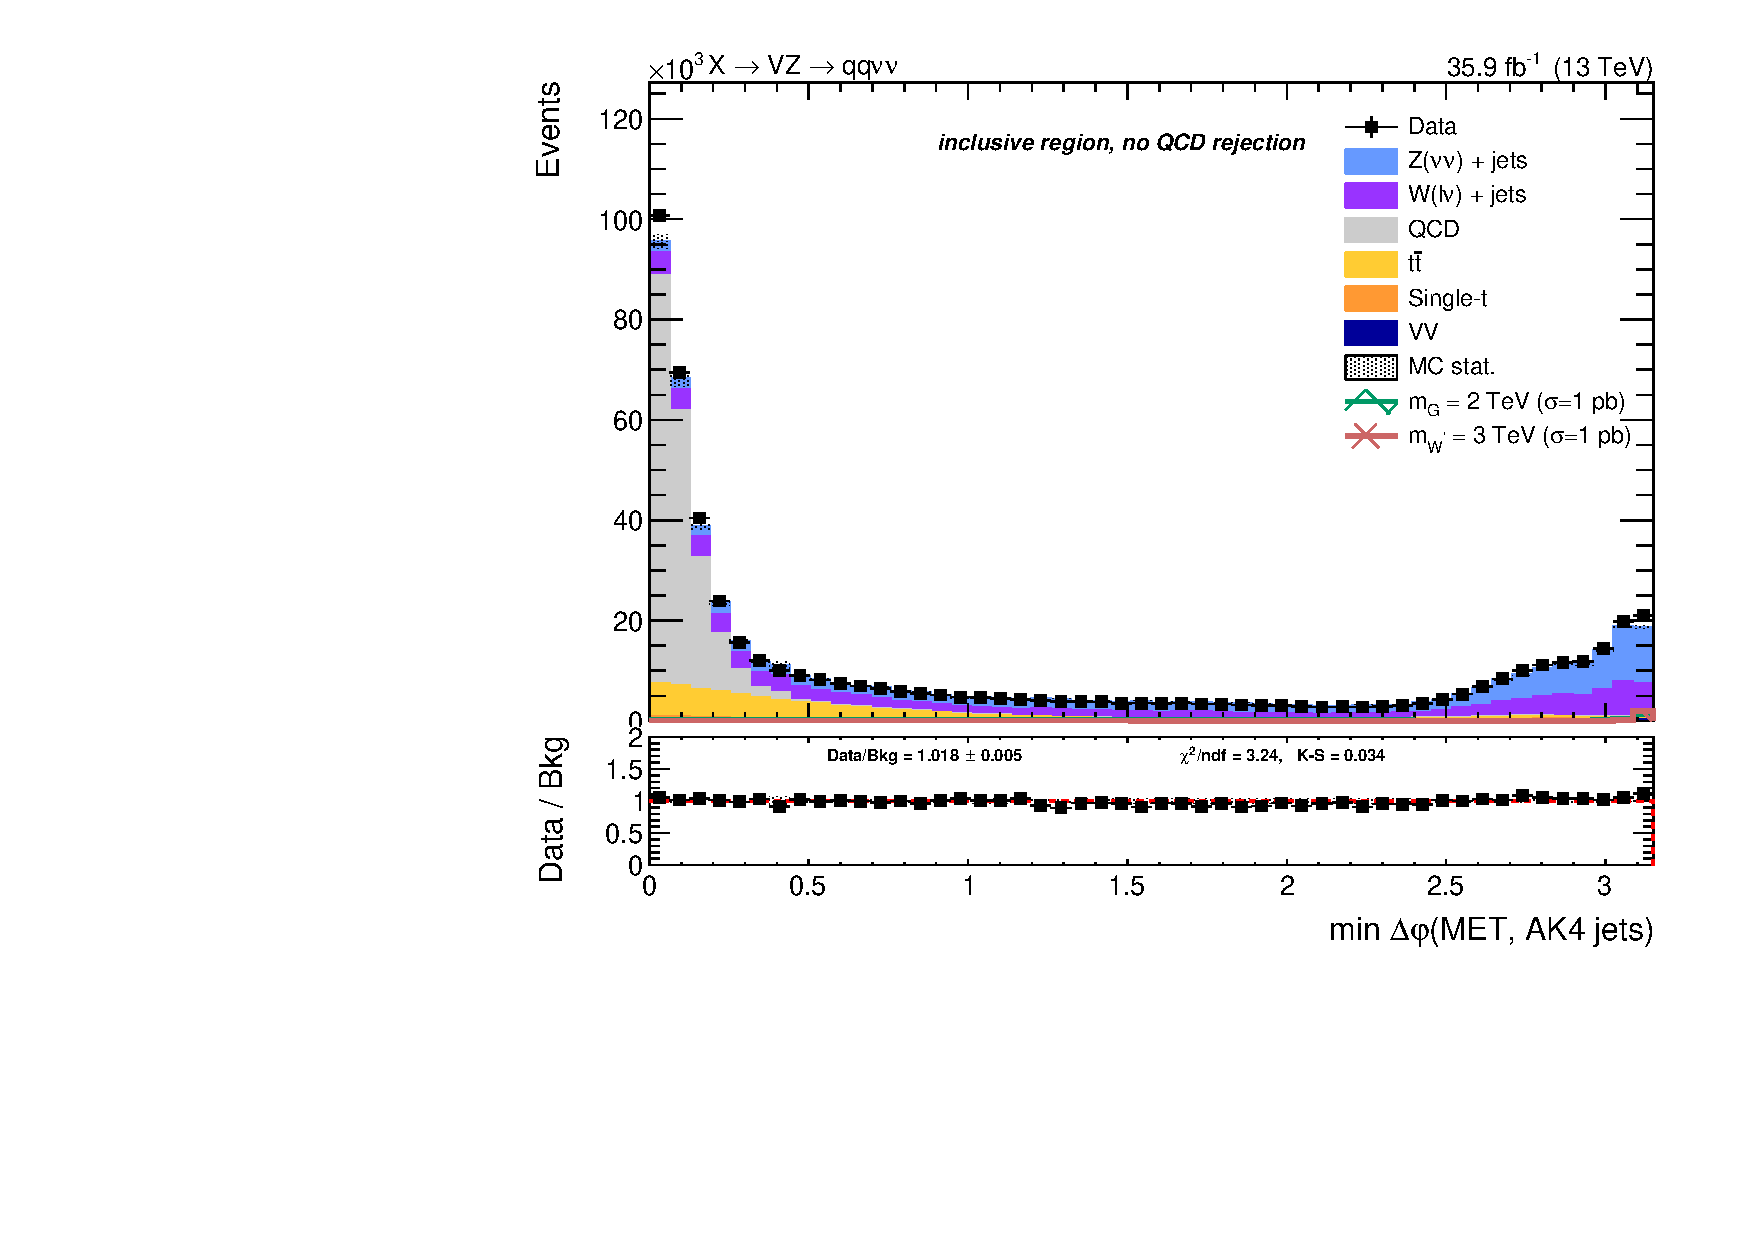
\includegraphics[width=.495\textwidth]{plots/v9_thesis/XVZnnNoQCDButPrunedMass/MinJetMetDPhi.pdf}
  \caption{Distribution of the minimum azimuthal separation bewteen \met and the momenta of all the AK4 jets present in each event. By imposing $\text{min} \Delta \varphi > 0.5$, the QCD background (in gray) is suppressed.}
  \label{fig:QCD_cleaning}
\end{figure}

\vspace*{1\baselineskip}

\noindent The final selections of the analysis are summarized in tab.~\ref{tab:sel}-\ref{tab:categorization}. The detection efficiencies due to each cut sequentially applied to bulk graviton signal samples (fig.~\ref{fig:eff_n}, left) and \Wp signal samples (fig.~\ref{fig:eff_n}, right) are shown. The signal efficiency for bulk graviton ranges from $\sim 30 \%$ at 1 \TeV, down to 20\% at 4.5 \TeV for low-purity category, whilst it's around 20\% for the high-purity category in the whole mass range. The signal efficiency for \Wp ranges from $\sim 40 \%$ at 1 \TeV, down to 25\% at 4.5 \TeV for low-purity category, whilst it's around 25\% for the high-purity category in the whole mass range. The different detection efficiencies for the two signals are related to their production mechanisms: the graviton is produced in gluon fusion, hence more hadronic activity is expected around the \VZ decay process, and this results as a loss of efficiency when the QCD rejection cut is applied.

\begin{table}
\centering
  \caption{Summary of the selection cuts for the $\VZ \to q \bar{q} \nu\bar{\nu}$ analysis.}
\begin{tabular}{l|c}
 & $\VZ \to q \bar{q} \nu\bar{\nu}$ \\
\hline
\hline
Trigger & \texttt{HLT\_PFMETNoMu90\_PFMHTNoMu90\_IDTight}\\
&  or \texttt{HLT\_PFMETNoMu110\_PFMHTNoMu110\_IDTight}\\
& or \texttt{HLT\_PFMETNoMu120\_PFMHTNoMu120\_IDTight} \\
& or \texttt{HLT\_PFMET170\_NoiseCleaned} \\
& or \texttt{HLT\_PFMET170\_JetIdCleaned} \\
& or \texttt{HLT\_PFMET170\_HBHECleaned}\\
\hline
$E_T^{\text{miss}}$ & \emph{Type-I} corrected\\
 & $>200$ \GeV\\
\hline
Veto & $e$, $\mu$, $\tau$, $\gamma$\\
\hline
\V & $p_T>200$ \GeV, \emph{tight} Id\\
 &  nhf$<$0.8; chf$>$0.2\\
\hline
QCD cleaning & $\text{min} \Delta \varphi(\text{AK4jets},\met)>0.5$ \\
Top cleaning & veto on b-tagged AK4 jets outside the AK8 cone, \emph{loose} working point ($<0.460$)\\
Event cleaning & $\Delta\varphi(\V,\met)>2$\\
%\hline
%\hline
%V mass  & SR: $65<m_V<105$\\
% &  SB: $30<m_V<65$, $m_V>135$ \GeV\\
%\hline
%V $\tau_{21}$  & $0.35<\tau_{21}<0.75$ for low-purity\\
% &  $\tau_{21}<0.35$ for high-purity\\
  \end{tabular}

  \label{tab:sel}
\end{table}

\begin{table}
\centering
  \caption{Cuts to categorize the $\VZ \to q \bar{q} \nu\bar{\nu}$ analysis events into low- and high-purity categories, and into signal region and sidebands.}
\begin{tabular}{l|c}
 & $\VZ \to q \bar{q} \nu\bar{\nu}$ \\
\hline
\hline
V mass  & Signal Region: $65<m_V<105$\\
 &  Side Bands: $30<m_V<65$, $m_V>135$ \GeV\\
\hline
V $\tau_{21}$  & $0.35<\tau_{21}<0.75$ for low-purity\\
 &  $\tau_{21}<0.35$ for high-purity\\
  \end{tabular}

  \label{tab:categorization}
\end{table}



\begin{figure*}[!hbtp]\centering
  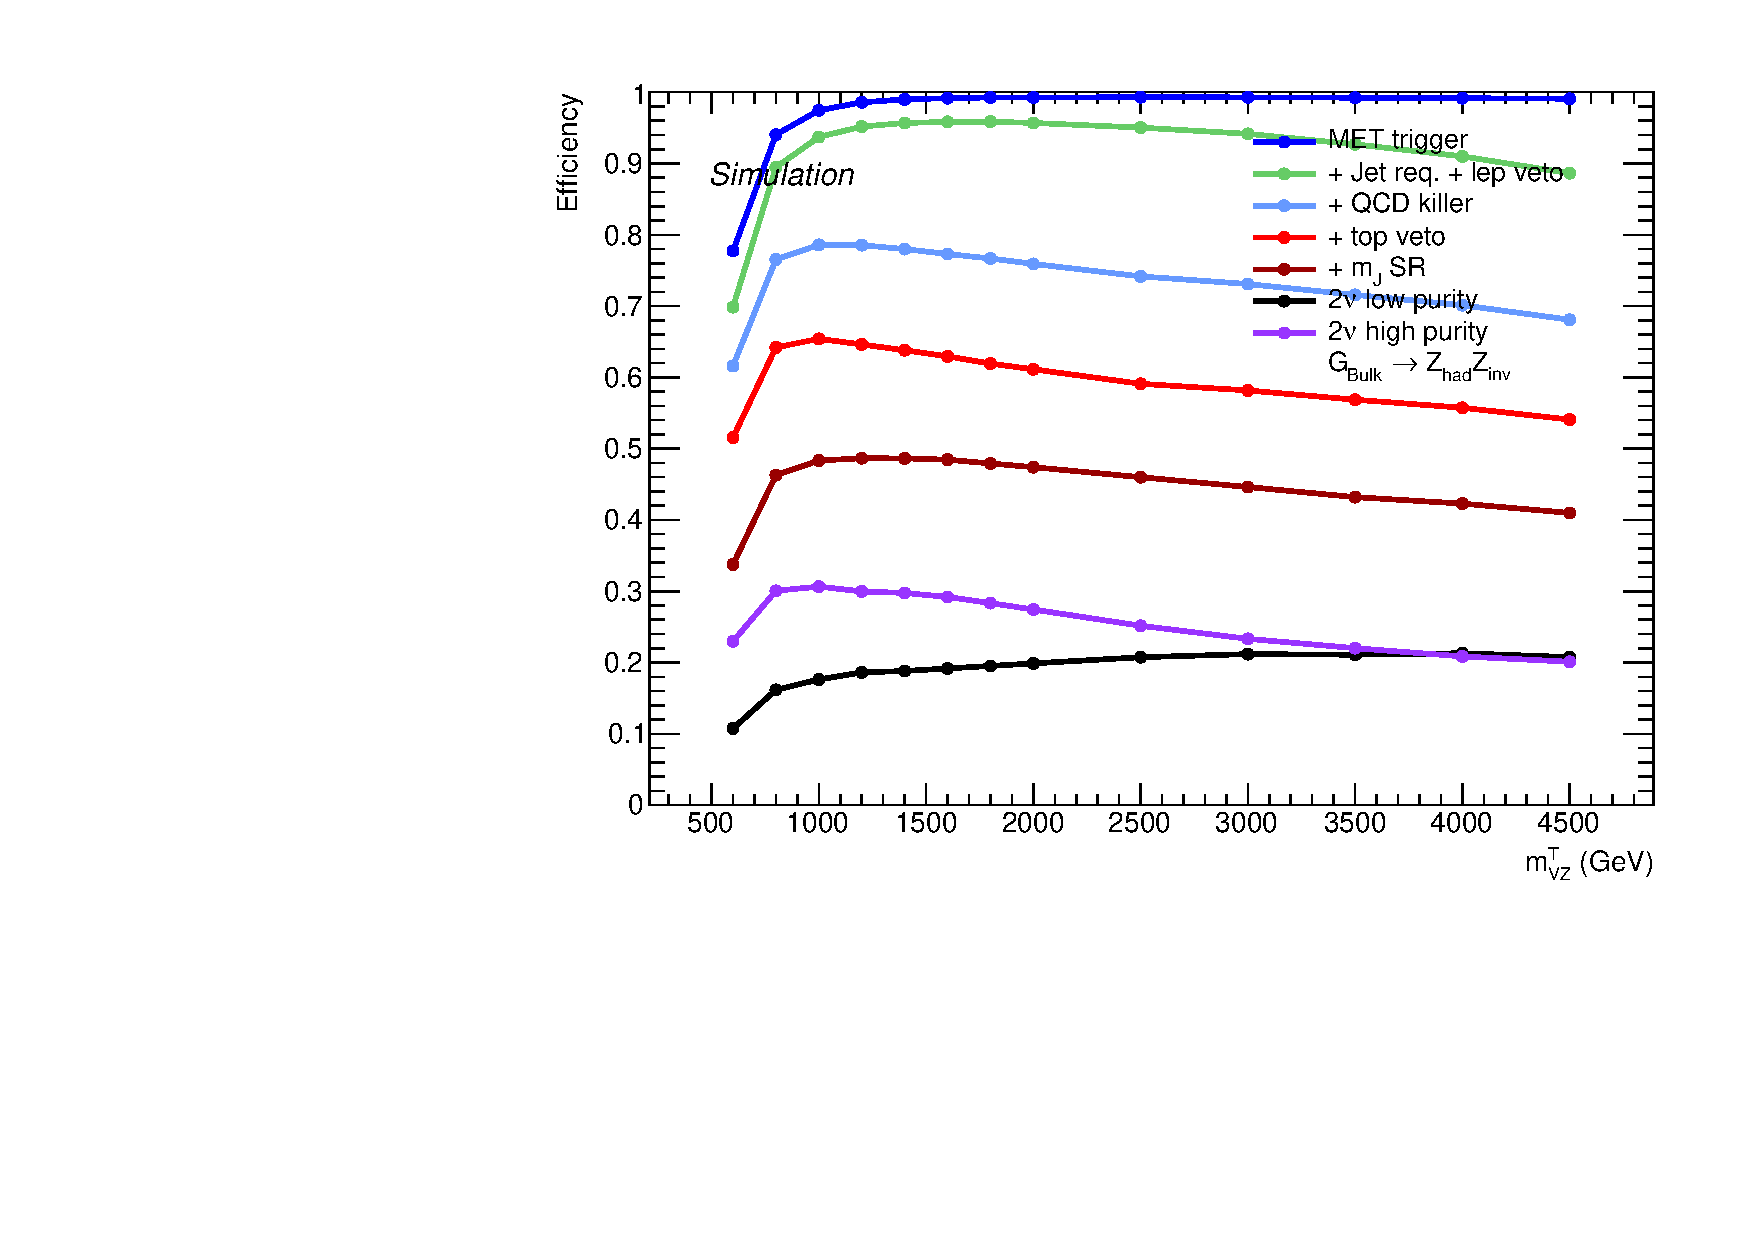
\includegraphics[width=0.5\textwidth]{ZhadZinv_thesis/Efficiency_v9_XZZInv.pdf}%
  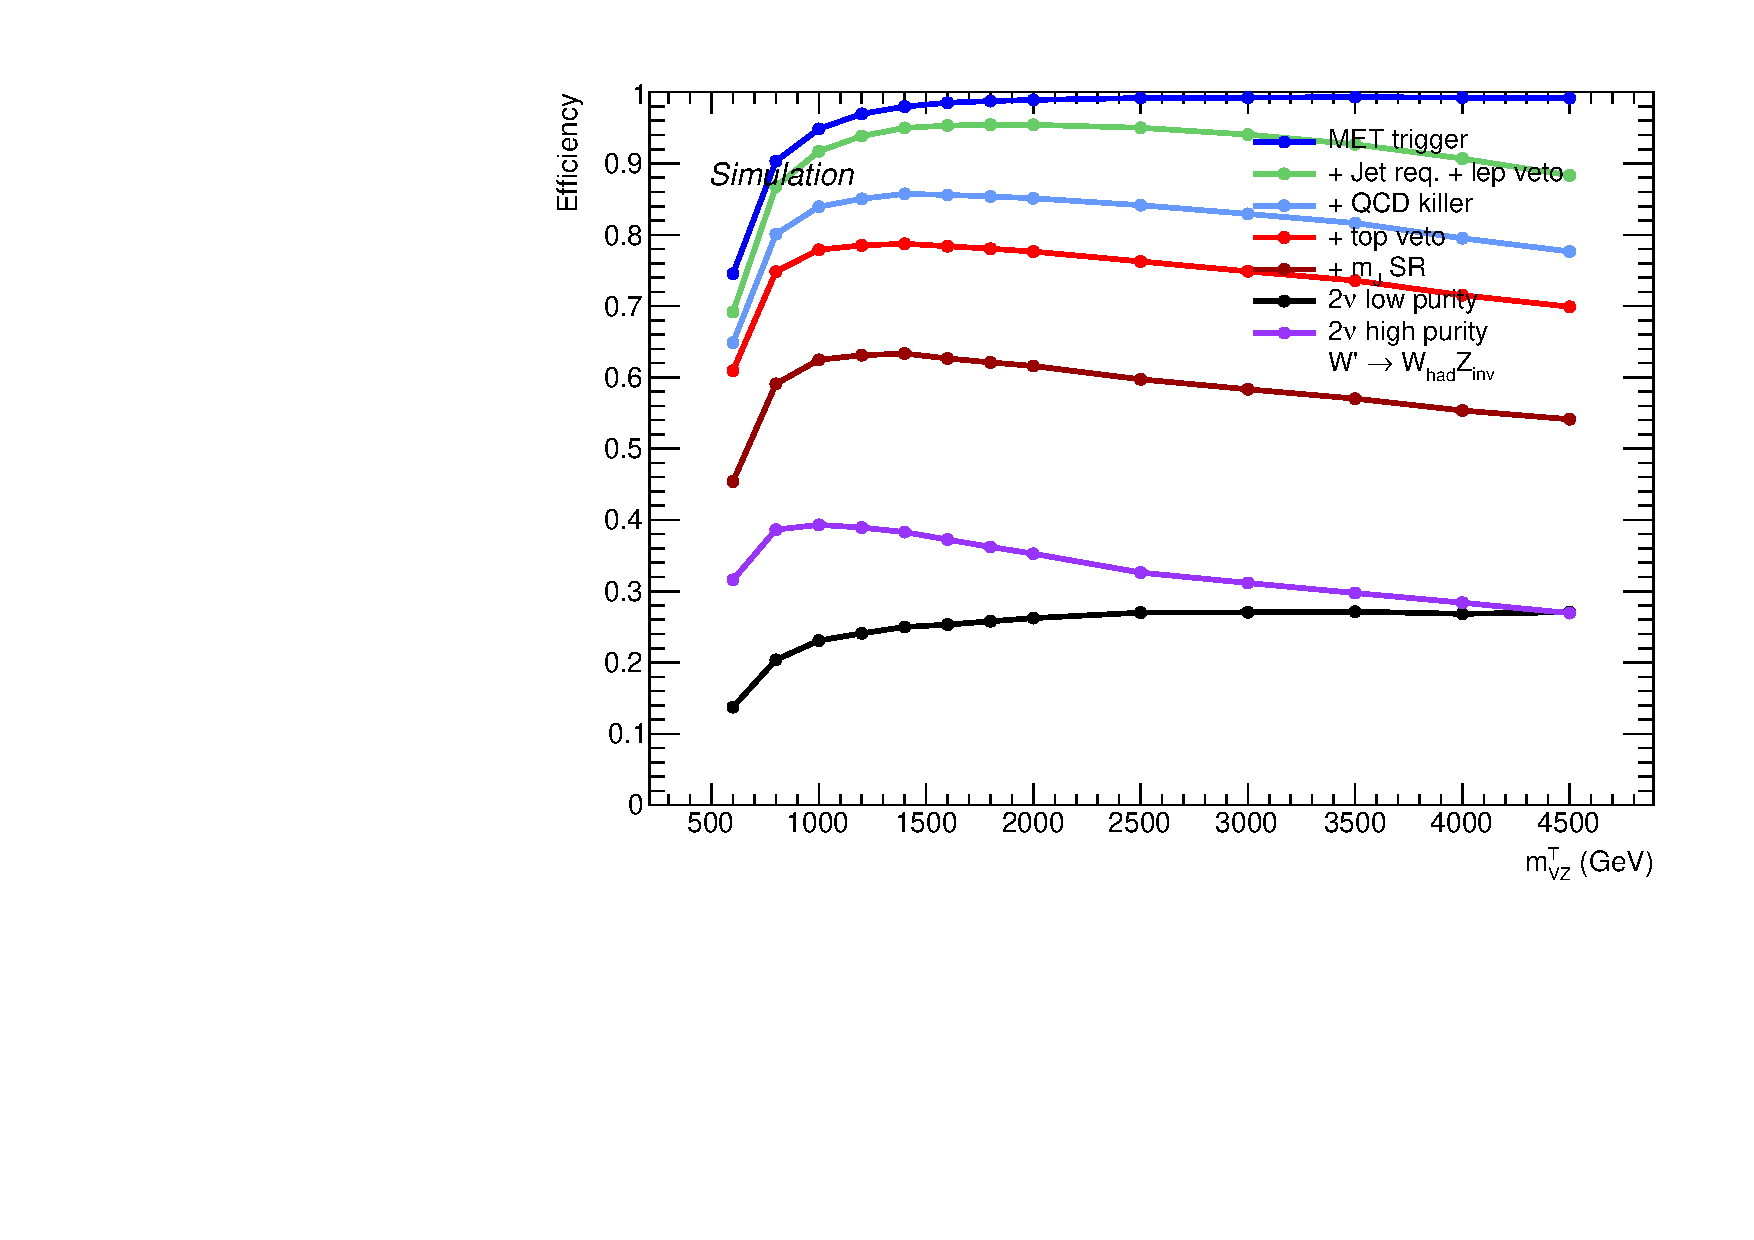
\includegraphics[width=0.5\textwidth]{ZhadZinv_thesis/Efficiency_v9_XWZInv.pdf}
\label{fig:eff_n}
  \caption{Signal efficiency for a spin-2 bulk graviton decaying into a pair of \Z bosons (left), and for a spin-1 \Wp decaying into a \W and a \Z bosons (right), as a function of the mass of the heavy particle. The efficiencies are separated by purity category after the signal region selections.}
\end{figure*}


\clearpage
